\documentclass[14pt,a4paper]{article}
\usepackage[warn]{mathtext}
\usepackage[utf8]{inputenc}
\usepackage[T2A]{fontenc}

\usepackage[english,russian]{babel}
\usepackage{multicol}
\usepackage{fancyhdr}
\usepackage{graphicx}
\usepackage{microtype}
\usepackage{wrapfig}
\usepackage{amsmath}
\usepackage{floatflt}
\usepackage{pdfpages}
\usepackage{geometry} \geometry{verbose,a4paper,tmargin=2cm,bmargin=2cm,lmargin=1.5cm,rmargin=1.5cm}
\usepackage{float}
\usepackage{amssymb}
\usepackage{caption}
\usepackage{epsfig}
\usepackage{newunicodechar}
\newcommand{\angstrom}{\textup{\AA}}

\usepackage{indentfirst}
\usepackage{misccorr}
\usepackage{subcaption}
\captionsetup{compatibility=false}
\usepackage{wrapfig}
\usepackage{amsmath}
\usepackage{float}
\usepackage{amssymb}
\usepackage{color}
\usepackage{lscape}
\usepackage{hvfloat}
\usepackage{amsfonts}
\usepackage{euscript}
\usepackage{textcomp}
\usepackage{mathtext}
\usepackage{latexsym}
\usepackage{xcolor}
\usepackage{hyperref}
\usepackage{booktabs}
\usepackage[version =3]{mhchem}
\usepackage{commath}
\usepackage{gensymb}
\usepackage{fancyhdr}
\usepackage[normalem]{ulem}
\newcommand{\RomanNumeralCaps}[1]
    {\MakeUppercase{\romannumeral #1}}

\definecolor{linkcolor}{HTML}{000BFF} % цвет ссылок
\definecolor{urlcolor}{HTML}{000BFF} % цвет гиперссылок

\begin{document}

    \graphicspath{\pictures}
    \pagenumbering{arabic}

\begin{center}
    {\scshape\Large Задачи к экзамену по Квантовой Оптике} \par

    {\large Яромир Водзяновский Б04-855а}
\end{center}

\section*{Задача 1}
    
    \par \textbf{Найти длины волн (мкм), частоты (Гц) и энергии(эВ) для 7 цветов диапазона, видимого глазом человека излучения.}\\
    
    \par 
        \begin{enumerate}
            \item Красный\\
            длина волны {$\lambda$}: 690 нм\\
            частота {$\nu$}: {$4,35 \cdot 10^{14}$} Гц\\
            энергия {$\hbar \omega$}: 1,8 эВ
            \item Оранжевый\\
            длина волны {$\lambda$}: 610 нм\\
            частота {$\nu$}: {$5,00 \cdot 10^{14}$} Гц\\
            энергия {$\hbar \omega$}: 2,0 эВ
            \item Жёлтый\\
            длина волны {$\lambda$}: 580 нм\\
            частота {$\nu$}: {$5,02 \cdot 10^{14}$} Гц\\
            энергия {$\hbar \omega$}: 2,1 эВ
            \item Зелёный\\
            длина волны {$\lambda$}: 530 нм\\
            частота {$\nu$}: {$5,70 \cdot 10^{14}$} Гц\\
            энергия {$\hbar \omega$}: 2,3 эВ
            \item Голубой\\
            длина волны {$\lambda$}: 490 нм\\
            частота {$\nu$}: {$6,12 \cdot 10^{14}$} Гц\\
            энергия {$\hbar \omega$}: 2,5 эВ
            \item Синий\\
            длина волны {$\lambda$}: 460 нм\\
            частота {$\nu$}: {$6,52 \cdot 10^{14}$} Гц\\
            энергия {$\hbar \omega$}: 2,7 эВ
            \item Фиолетовый\\
            длина волны {$\lambda$}: 420 нм\\
            частота {$\nu$}: {$7,10 \cdot 10^{14}$} Гц\\
            энергия {$\hbar \omega$}: 3,0 эВ
        \end{enumerate}

\vspace{0.8cm}

\section*{Задача 2}
    
    Закон Вина: $\lambda_m T = const = 0.002898 \; m\cdot k$

    $$t_1 = 40 ^{\circ} C = 313\; K$$
    $$ \lambda_{m_1} = 0.259 \; mkm $$
    $$ t_2 = 6000 ^{\circ} C = 6273\; K $$
    $ \lambda_{m_2} = 462\; nm $ — соответсвует зеленому свету с пиком спектра слонца, поэтому бильярдный стол зеленый.
  
\vspace{1cm}

\section*{Задача 3}
    
    \par \textbf{Оценить суммарную мощность излучения (Вт), испускаемую Вами при нормальной температуре (t = $36,6^{\circ}$ C) и в состоянии болезни (t = $42^{\circ}$ C).}\\

    \par

    Закон Стефана-Больцмана:

    $$ J = \sigma T^4 $$
    $\sigma = 5.67\cdot 10^{-8} \; \frac{W}{m^2 K^4}$

    Площадь человеческого теля $S \approx 1.8\; m^2$

    $t_1 = 46.6 ^{\circ} C = 309.75\; K \Rightarrow W_1 = J_1 S = \sigma T_1^4S = 940\; W$
    \par 
    $ t_2 = 42 ^{\circ} C \Rightarrow W_2 = 1007\; W $
    
\section*{Задача 4}
    
    \par \textbf{При классическом представлении Э-М поля, при какой его плоской поляризации (в плоскости падения или перпендикулярно ей) выход фотоэлектронов будет больше при всех равных других параметров излучения и фотокатода.}\\
    
    \par

    Эффект будет сильным, если электрическое поле перпендикулярно плоскости падени: в этом случа проекция поля на катод максимальна.
    
\section*{Задача 5}
    
    \par \textbf{Определите красную длину волны фотоэффекта на алюминиевом фотокатоде, найдя его работу выхода. Найдите {$E_{MAX}$} фотоэлектрона, выбитого из алюминиевого фотокатода 4-ой гармоникой лазера на неодиме.}\\
    
    \par 

    $$A_{out} = 4.25\; eV \Rightarrow \lambda_{red} = \frac{h e}{E} = \frac{6.83 \cdot 10^{-34} 3 \cdot 10^8}{4.25 \cdot 10^{-19} \cdot 1.6} = 292.5\; nm$$
    
    Первая гармоника неодимового лазера: $\lambda_n = 106\; nm$. Длина волны 4-ой грамоники: $\lambda_{n_4} = \frac{\lambda_n}{4} = 266\; nm$
    $$E = E_{em} - A_{out} = \frac{hc}{\lambda_{n_4}} - A_{out} = 0.42\; eV$$

\section*{Задача 6}
    
    \par \textbf{Постройте линейную функцию запирающего потенциала от частоты падающего на фотокатод излучения {$U_{\hbox{зап}} = kV + b$}. Выразите k и b через константы и параметры фотокатода и покажите их на графике.}\\
    
    \par 

    $U_{cl} = h \nu + b$, $h \nu = A + \frac{m \upsilon^2}{2} = A + eV_{cl}$
    $$V_{cl} = \frac{h}{e}\upsilon - \frac{A_{out}}{e}$$
    $k = \frac{h}{e},\; b = -\frac{A_{out}}{e}$

    \begin{figure}[H]
        \begin{center}
            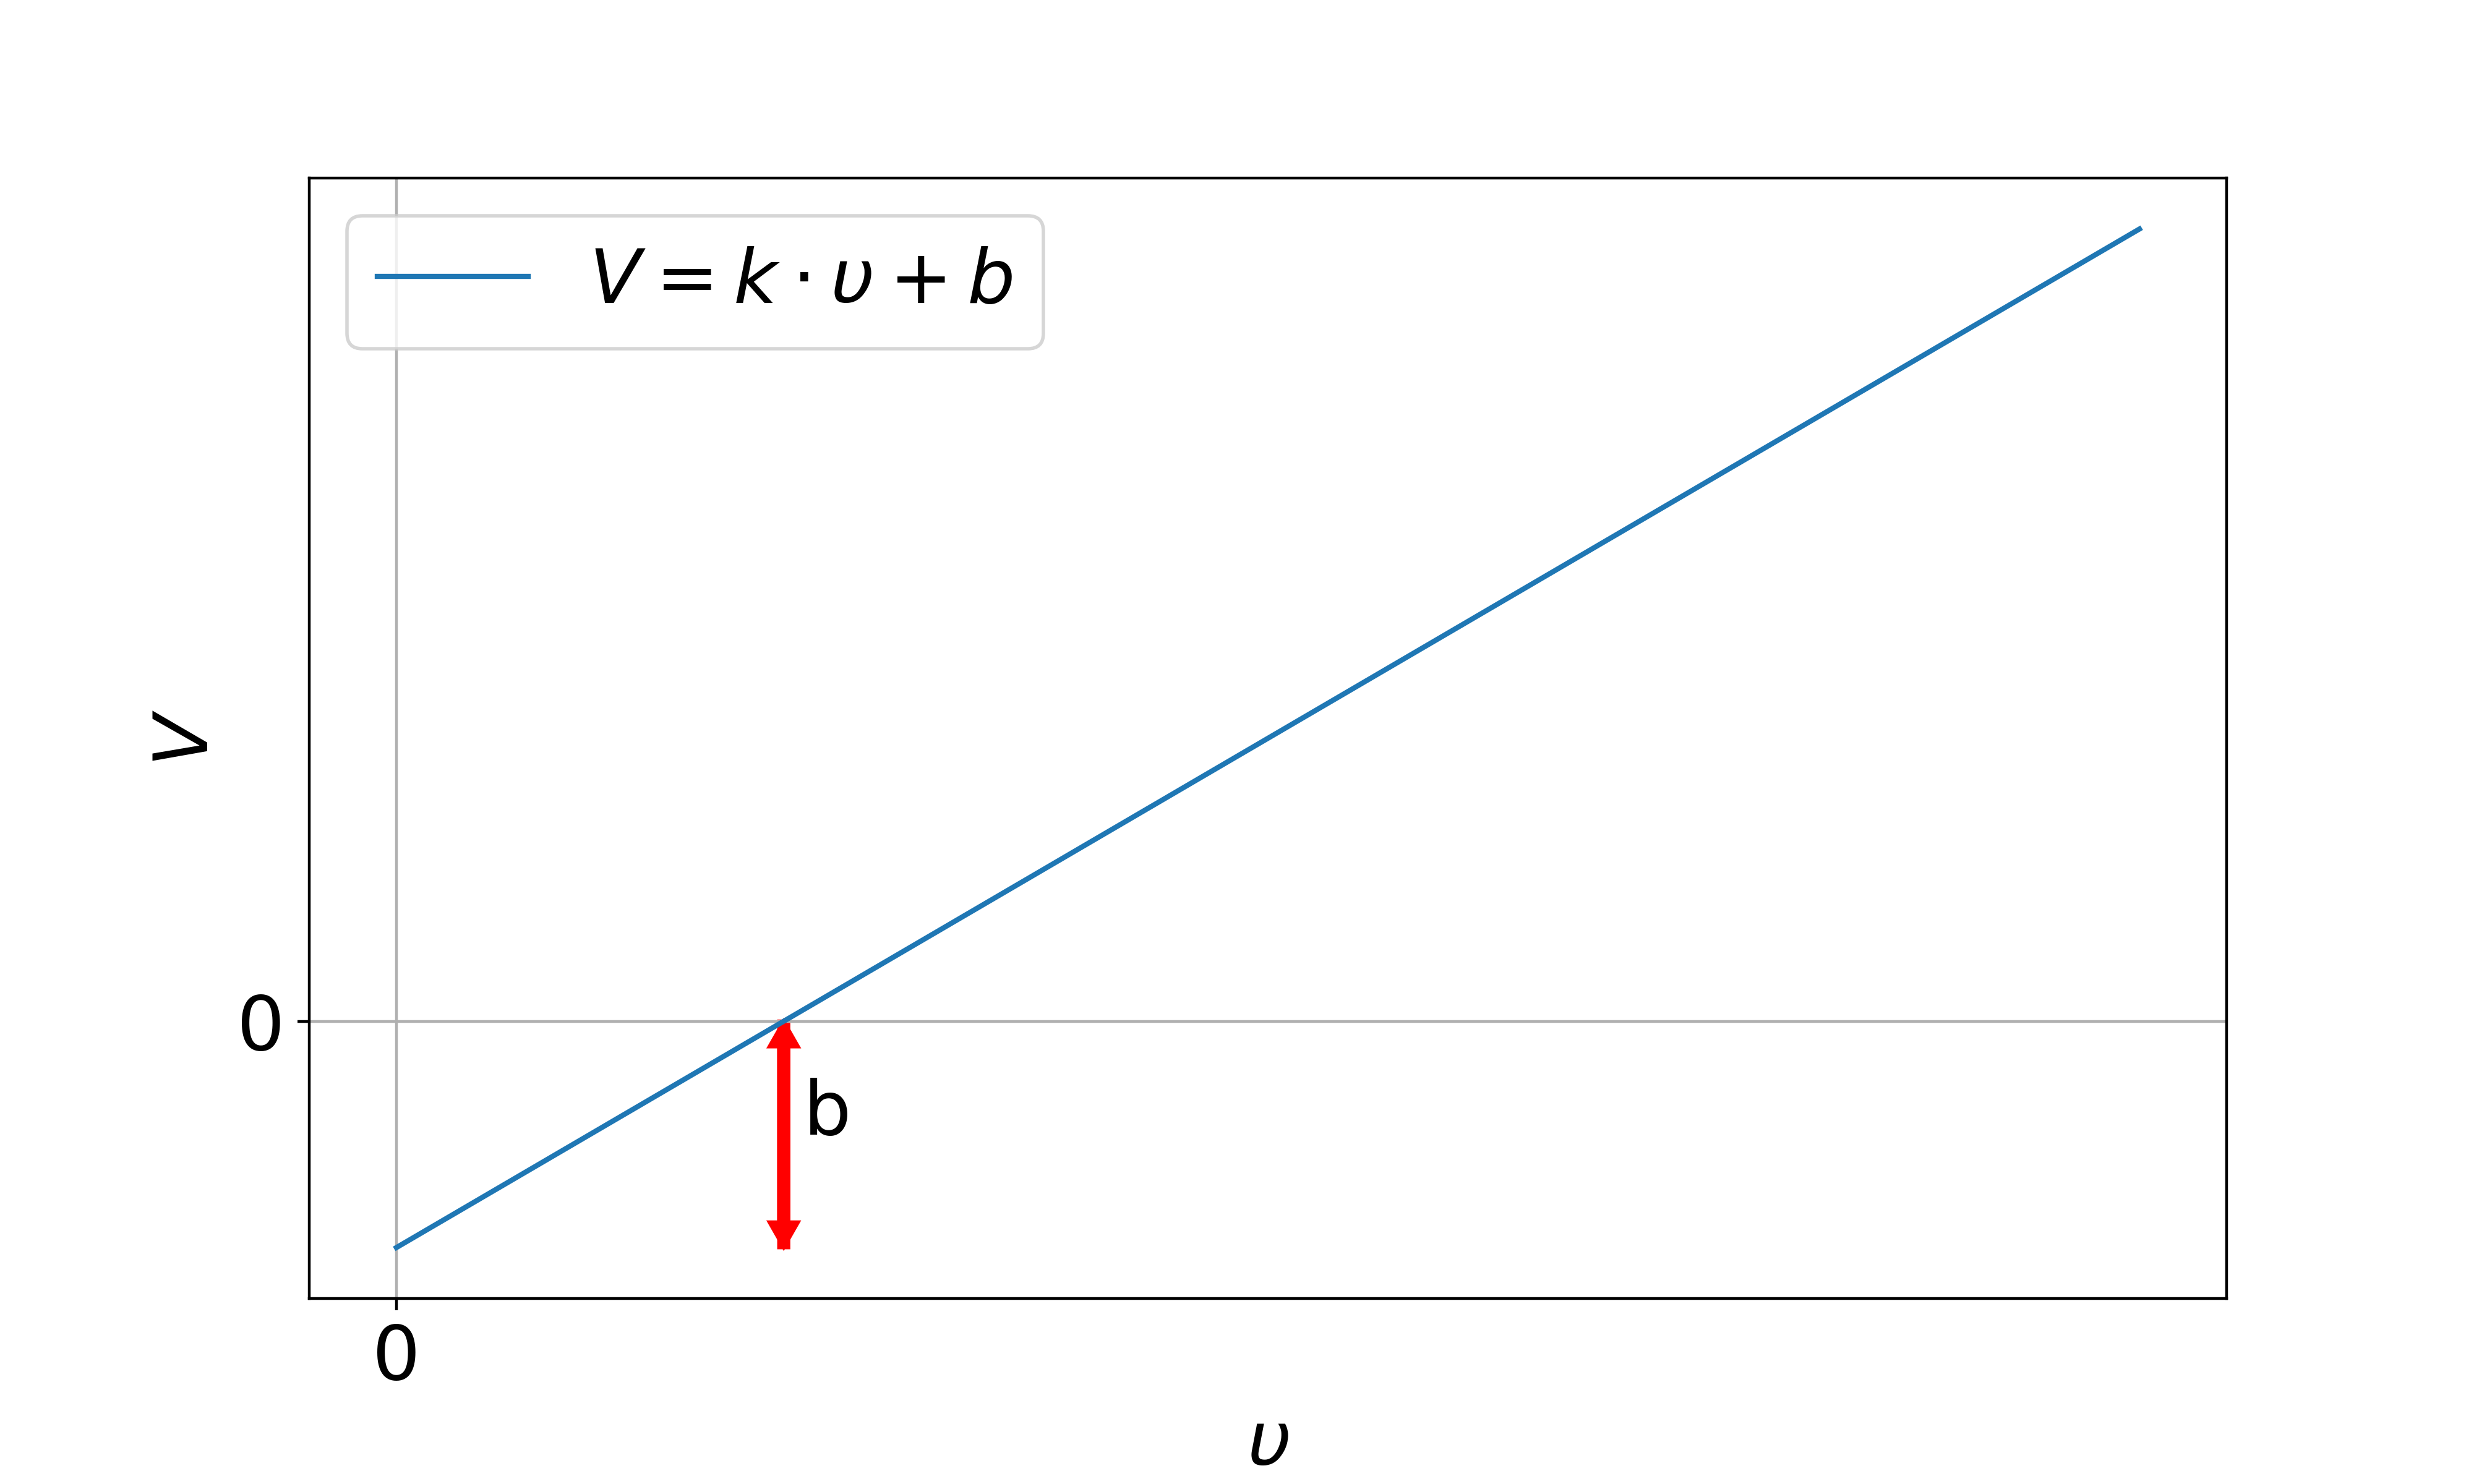
\includegraphics[scale=0.5]{task_6.png}
            \caption{}
            \label{fig:task_6}
        \end{center}
    \end{figure}

\section*{Задача 7}
    
    \par \textbf{Покажите, что поглощение / излучение свободного фотона свободным электроном - процесс, запрещенный законами сохранения.}\\

    \par 

    СО связана с электроном:

    \begin{equation}
        \begin{cases}
            0 = \frac{m \vec{\upsilon}}{\sqrt{1 - \frac{\upsilon^2}{c^2}}} + \vec{p_{ph}} \\
            mc^2 = \gamma mc^2 + |p_{ph}|c \\
        \end{cases}
    \end{equation}

    $\vec{p}_{ph} = -\gamma m \vec{\upsilon}$

    $mc^2 = \gamma m c^2 + \gamma mc |\vec{\upsilon}|$; $c = \gamma c + \gamma |\vec{\upsilon}|$

    $c = \gamma c + \gamma |\vec{\upsilon}|$

    $c = \frac{\gamma |\vec{\upsilon|}}{1-\gamma}$

    $\gamma \in [1, + \infty)\;; \upsilon = p \Leftrightarrow \gamma=1$

    Значит, что единственное решение $\vec{\upsilon} = 0$, но тогда $p_{ph} = 0$ (не было фотона) и процесс завершен, аналогично для поглощения.

\section*{Задача 8}
    
    \par \textbf{Определите изменение длины волны излучения при рассеянии его на пучке встречных релятивистских электронов, считая, что в результате неупругого столкновения с фотоном электрон часть своей кинетической энергии передал фотону, который отразился назад от релятивистского зеркала налетающих электронов.}\\
    
    \par при обратном эффекте Комптона энергия фотонов:\\
    
    {$E^{\gamma}_{MAX} = E_{0} \frac{E^{\gamma}_0 E_0}{4 E^{\gamma}_0 E_0 + m^2 c^4}$}\\
    
    \par где {$E^{\gamma}_0$} - начальная энергия излучения, {$E_0$} - энергия электронов\\
    
    {$\Delta \lambda = \lambda' - \lambda = \frac{hc}{E^{\gamma}_{MAX}} - \frac{hc}{E^{\gamma}_0}$}\\

\section*{Задача 9}
    
    \par \textbf{Найдите и запишите выражения для вариационного принципа Ферма для оптики и вариационного принципа Мопертюи-Лагранжа для механики массовой частицы. Сравните их и попробуйте найти аналогии.}\\
    
    \par 
    Принцип Ферма: из множества возможных путей свет идет по тому, который занимает меньше всего времени. \par 
    Принцип Мюпертюи-Лагранжа: принцип наименьшего действия $\delta S = 0$. \par 
    Принципи по идее эквивалентны: $S = \int_{\delta S=0} L(q, \dot{q}, t) dq$

\section*{Задача 10}
    
    \par \textbf{Выпишите выражение для физической величины \textsc{действие} (S). Найдите ее размерность и сравните с размерностью постоянной Планка h. Запишите фазу плоской волны и фазу волновой функции через S/ h и сравните их временные и пространственные части.}\\
    
    \par 

    $\psi = A e^{\frac{i}{\hbar}} \hat{S}$ - волновая функция

    Классическое действие: $S = \int pdq - \int H dt$, размерности $S$ и $h$ совпадают

\section*{Задача 11}
    
    \par \textbf{Как по картинке миража понять на юге или на севере это происходит?}\\
    
    \par 

\section*{Задача 12}
    
    \par \textbf{Оцените период кристаллической решетки никеля, если дифракционная картина типа Лауэ или Брега происходит с электронами, разогнанными разностью потенциалов в 150 эВ.}\\
    
    \par 

    $E_e = 150\; eV$

    $2d = \lambda = \lambda_{D} = \frac{h}{p} = \frac{h}{\sqrt{2Em}} \approx 1 \angstrom$

    $d = 0.5 \angstrom$

\section*{Задача 13}
    
    \par \textbf{Вычислить спектральное фурье - преобразование от функция временной когерентности}\\
    
    \par 

    Функция когерентна. $\Gamma(\tau) = \lbrace E(t) E(t-\tau) \rbrace$

    $E(t) = \int_{-\infty}^{+\infty} a(\omega) e^{i \omega t} d \omega$

    $a(\omega) = \frac{1}{2 \pi} \int_{-\frac{\pi}{2}}^{+\frac{\pi}{2}} E(\varphi) e^{-i \omega t} dt $

    $ \Gamma(\tau) = \frac{1}{\tau} \int_{\frac{-\pi}{2}}^{\frac{\pi}{2}} E(t) E(t-\tau) dt = \frac{1}{\tau} \int_{-\infty}^{+\infty} a^*(\omega) e^{i \omega \tau}
    \left ( \int_{\frac{-\pi}{2}}^{\frac{\pi}{2}} E(t) e^{-i \omega t} dt \right ) = \int_{-\infty}^{+\infty} F(\omega) e^{i \omega t} d \omega$ 

    $F(\omega) = \int_{-\infty}^{+\infty} \Gamma(\tau) e^{-i \omega \tau} d \tau $

\section*{Задача 14}
    
    \par \textbf{Найти выражение для аксиальных мод пустого резонатора и константу из предыдущего равенства для пустого резонатора длины L.}\\
    
    \par 
    Для пустого резонатора: $k_n L = 2 \pi n \Rightarrow k_n = \frac{2 \pi n}{L},\; \lambda = \frac{2 \pi}{k}$

    $\lambda_n = \frac{2 \pi L}{2 \pi n} = \frac{L}{n}$

\section*{Задача 15}
    
    \par \textbf{Оценить длину продольной когерентности излучения АЧТ в
длинах волн для комнатной температуры и для температуры короны Солнца.}\\
    
\par T = 300 K, {$\lambda_m = 9666$} нм\\

{$\lambda_2 = 17500$} нм {$\rightarrow \lambda_1 = 5900$} нм\\

{$l = \frac{\lambda}{\Delta \lambda} \lambda \approx 0,8 \lambda$}\\

\par T = $10^6$ K, {$\lambda_m = 2,9$} нм\\

{$\Delta \lambda = 3,53$} нм\\

{$l = \frac{2,9}{3,53} \lambda \approx 0,8 \lambda$}

\section*{Задача 16}
    
    \par \textbf{Оценить плотность мощности излучения, создаваемую
лазером на АИГ + Nd, имеющего диаметр выходной диафрагмы 2 мм и мощность импульса 100мДж на мишени на расстоянии 5 км.}\\
    
    \par 

    d = 2mm, W = 100 mJ, L = 5 km, $\lambda = 1064\; nm$, $\theta = \lambda / d$

    $R/L = \tan{\theta} \Rightarrow R = L \tan{\theta}$

    $D = 2R = 2L \tan{\frac{\lambda}{d}}$

    $P = \frac{W}{S} = \frac{W}{2L \tan{\frac{\lambda}{d}}} = 4.5\; \frac{mJ}{m^2}$


\section*{Задача 17}
    
    \par \textbf{Найти температуру АЧТ, при которой параметр вырождения его излучения равен единице в видимом диапазоне.}\\
    
    \par

    $\delta = 1$  для оптического диапазона, $u \approx 0.5$

    $\delta = \frac{1}{e^{\frac{\hbar \omega}{kT}} - 1} = 1$

    $ e^{\frac{\hbar \omega}{kT}} = 2 \Rightarrow T = \frac{h c}{\lambda k \ln{2}} = 41600\; K$



\end{document}